\documentclass[11]{article}

\usepackage{graphicx}
\usepackage{hyperref}
\usepackage{subcaption}
\usepackage{amsmath}
\usepackage[
    backend=bibtex,
%    isbn=false,
%    url=false,
%    doi=false,
%    eprint=false,
%    hyperref=false,
%    backref=false,
%    firstinits=false,
]{biblatex}
\bibliography{references}

\hypersetup{colorlinks,urlcolor=blue}
\let \shorttitle \textbf
\begin{document}

\section{Introduction}
Tool use is one of the human abilities that uniquely distinguishes man from other species. 
We refer to tools as hand held devices employed in making changes to the surrounding environment. 
Cases of tool use have been reported in other species, but never to the extent engaged by humans \cite{boysen1999,harrington2009,lefebvre2004}. 
As a defining attribute of human cognition, we wish to lay the foundations for a computational model of tool use reasoning.

Our model stems from the architectural framework defined by the four constraints theory (4CT) \cite{osiurak2014a}.
In the following we describe 4CT with its implications in forming a computational model.  

\subsection{The four constraints theory}
4CT defines tool use behaviour of healthy individuals based on the empirical investigation of aprxia.
Apraxia is a neurological disorder impairing a person's ability to plan and execute sequences of movements.
The term covers a multitude of symptoms and levels of severity (e.g. dyspraxia, ideomotor aparaxia, apraxia of speech).
The underlying cause however is physical damage to the left hemisphere of the brain\cite{osiurak2013}.

\begin{figure}[h]
  \centering
  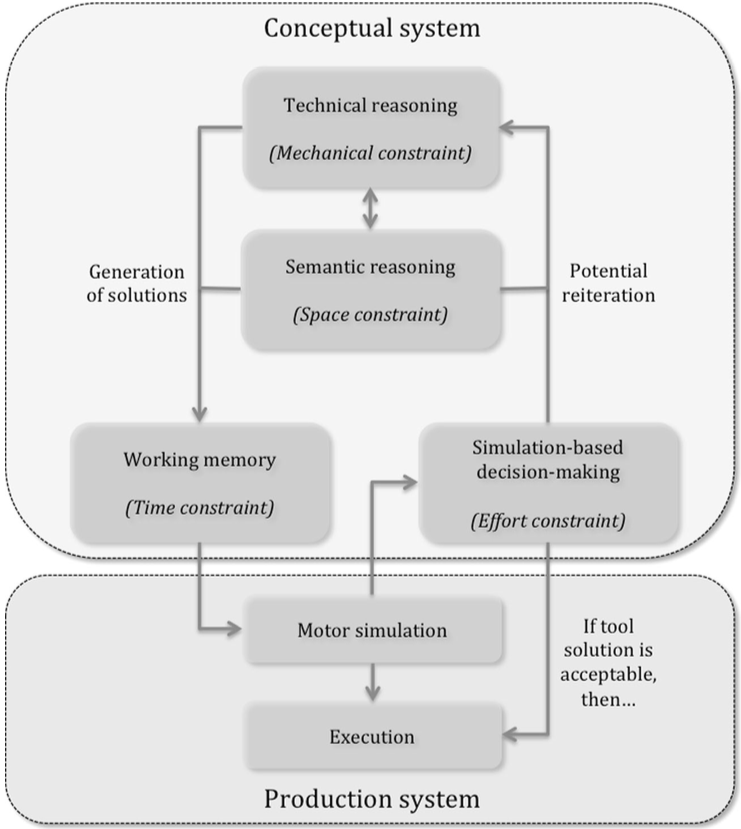
\includegraphics[width=.9\textwidth]{./figures/4CTArchitecture.png}
  \caption{4CT architecture reprinted from \cite{osiurak2014a}}
  \label{fig:4CTArchitecture}
\end{figure}      

Unlike competing theories, 4CT distinguishes between a conceptual and a production system when describing tool use(fig. \ref{fig:4CTArchitecture}).
Main focus is given to the conceptual system which encapsulates cognitive reasoning.
Further, the production system dictates movement by transforming a person's intent into motor control. 
By this distinction, 4CT's conceptual system is a suitable candidate for a model concentrated on reasoning.

%-----------
% More paragraphs needed to explain why 4CT is desired over other theories
%-----------

The theory characterises tool use situations as problem solving tasks requiring strong cognitive abilities. 
The four constraints of \emph{mechanics, space, time,} and \emph{effort} are the dimensions within which problems are defined.
Aiding problem solving are four cognitive processes: \emph{technical reasoning, semantic reasoning, working memory,} and \emph{simulation based decision making} (fig. \ref{fig:4CTArchitecture}).  
Even a simple scenario like slicing bread can be seen as reasoning about the knife's sharpness,length,serration and the movements necessary to manifest cutting effects. 

Problem solving becomes more apparent in the absence of familiar tools, when subjects are required to repurpose tools or fashion new ones.
A distinction is made between novel tool use and familiar tool use. 
Semantic reasoning refers to situations when subjects are accustomed with a tool's common purpose. 
For example a knife is used for cutting bread. 
The association is made on prior experience without considering the knife's physical properties.  
In novel cases however, technical reasoning is the inference of how the tool's properties can solve problems.
In the absence of a bread knife a saw would be a better cutting device than a spreading knife. 
Technical reasoning is a more general process for solving problems, but is more cognitively involved.  

The effort constraint and simulation based decision making refer to tool use energy cost. 
A simple rule of survival is that actions should require less energy than the rewards gained \cite{proffitt2006}.
Perceived effort would explain user's preference for one tool use method over another. 
Even when multiple tools are available, differences in their physical properties can lead to differences in effort which dictate choice. 

Working memory is required in the context where multiple steps must be fulfilled to achieve a goal. 
It describes a subject's ability to split activities into sub-goals and hold them in memory. 
Complex tasks such as fixing a radio would involve multiple steps and tool selection. 
However, such complex objectives are beyond the scope of this project.

A computational model should initially solve simple tool-use problems before complex ones.
Our focus is therefore on single step tool and object interaction involving generic situations.
These situations would be best solved through technical reasoning for its general problem solving abilities. 
However, beyond simple attributes such as object length,sharpness,abrasiveness, 4CT is not able to explain human decision-making.
Crucial factors of forces and geometric constraints are simply abstracted as mechanical knowledge. 
A computational model would therefore have to elaborate these items before fitting into the larger 4CT framework. 
The topic of this paper is solving geometric constraints through spatial reasoning in order to achieve simple tool-object interaction.  

\section{Experimental Setup}

Dietmar Heinke and Fran\c{c}ois Osiurak,the author of 4CT, have devised an experimental setup that tests human ability to use novel objects. 
The experiment is intended for use in both a computational model and to investigate human reasoning on tool and object geometries. 
Human trials were run in parallel to this project but do not constitute part of it. 
Nevertheless, this paper will refer to observed human behaviour even though data has not yet been published. 

\begin{figure}[!h]
  \centering
  \begin{subfigure}{0.49\textwidth}
    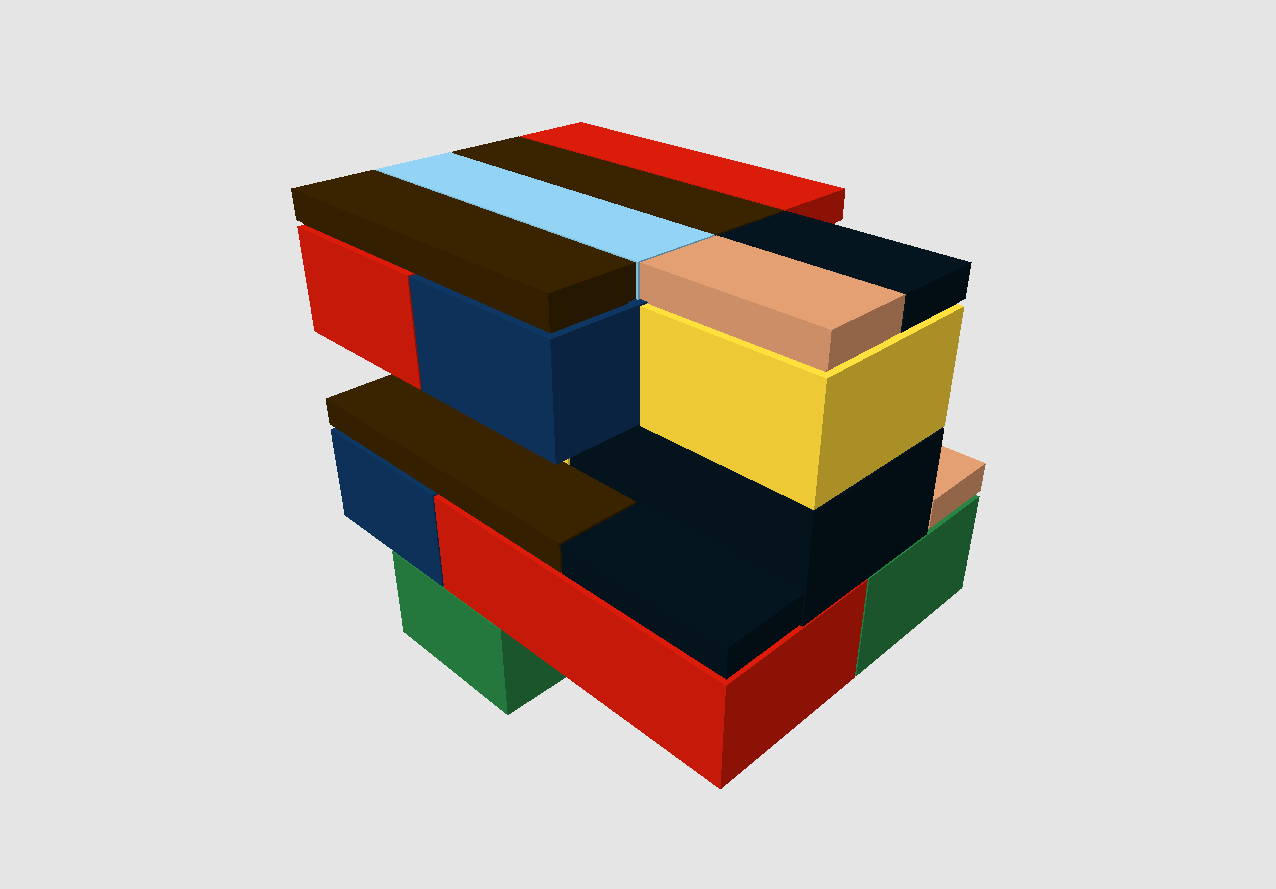
\includegraphics[width=1\linewidth]{./figures/obj51.png}
    \caption{Passive object}
    \label{fig:obj51}
  \end{subfigure}
  \begin{subfigure}{0.49\textwidth}
    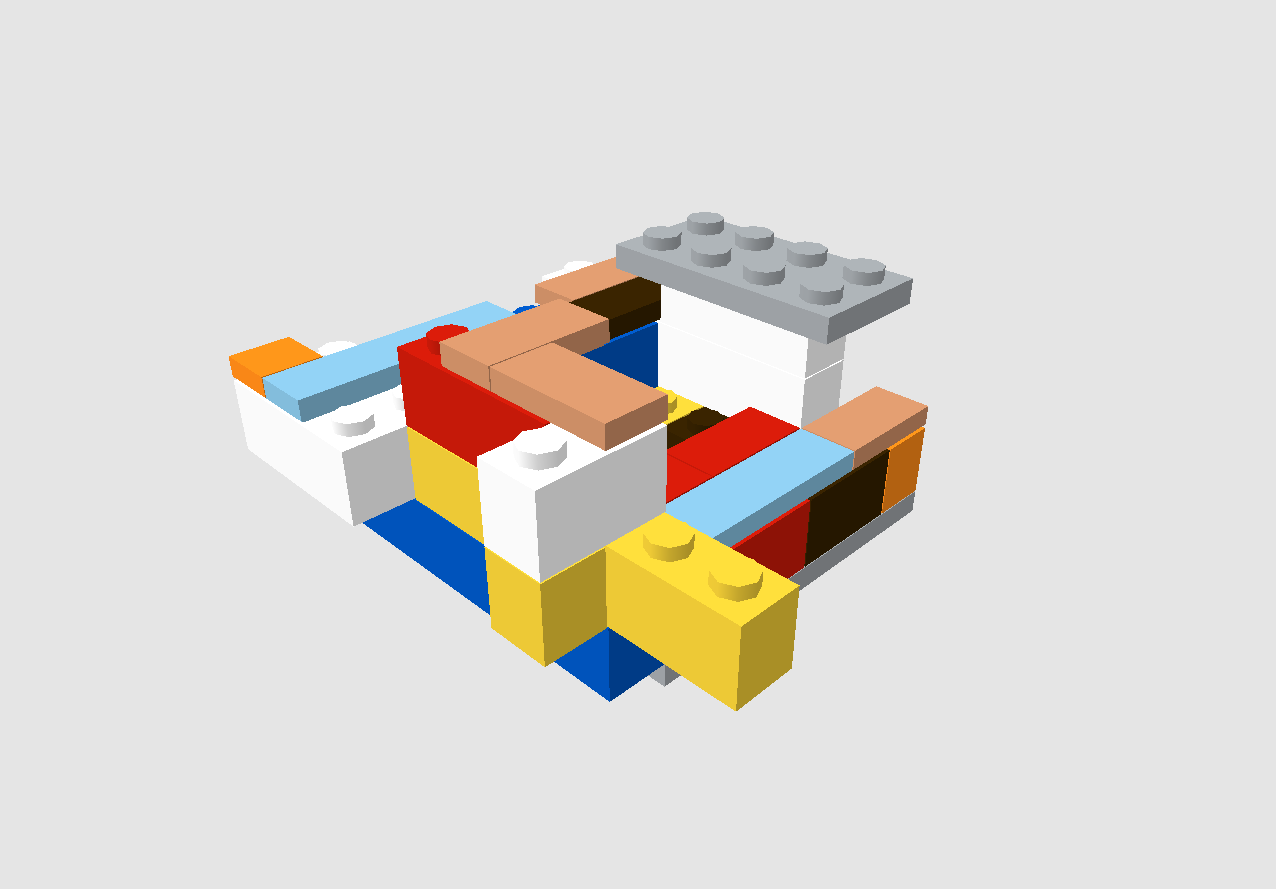
\includegraphics[width=1\linewidth]{./figures/obj52.png}
    \caption{Active object}
    \label{fig:obj52}
  \end{subfigure}
  \caption{Pair of novel tool and object models}
\end{figure}

A human subject is presented two novel objects composed out of LEGO blocks.
One object is passive and may not be directly touched (fig. \ref{fig:obj51}).
The second object is active and must be used to lift the passive object to a new location (fig. \ref{fig:obj52}).
As a tool use task, the active and passive objects are analogous to tool and target object.
Due to the unusual geometries, subjects must reason about the correct spatial fitting of tool and object.    

In summary, the experiment is a novel tool-object fitting task requiring spatial reasoning.
A computational model mimicking human behaviour, would solve geometric constraints similar to human subjects.

\section{Physics Engine Evaluation}

Formally solving object-tool fitting requires considerations of force closure.
However, a shortcut to computing forces and physical interaction is the use of a physics engine. 
To some extent, it is believed that the human brain computes approximate Newtonian laws \cite{battaglia2013}. 
Similarly, a physics engines does not compute exact friction, closure or gravity laws, but provides realistic alternative results. 
A tool use model can employ physics engines for one of multiple reasons:
\begin{enumerate}
      \item the engine can serve as source of inference over physical laws   
      \item it can verify solutions of tool-object fitting through simulation
      \item it is analogous to mental simulation (4CT)
\end{enumerate}

A suitable physics engine would satisfy the below criteria:
\begin{enumerate}
    \item The engine should have high fidelity in simulating rigid body collision. 
      That is, the engine should faithfully reflect real world interaction of bodies involving no moving parts or deformations.
      As tool and object are composed of LEGO, items are best represented as rigid bodies.   
      High fidelity is required to correctly evaluate tool-object fitting positions with minimal errors.
    \item The engine should be available in user-friendly scientific languages (such as Matlab or Python). 
      Scientific languages have many inbuilt algorithms that can be leveraged.
      Additionally, language difficulty shifts focus from the problem being solved to solving code complexities.
    \item There should be no associated fees or reduced cost for engine use.
    \item The engine should be portable to common platforms (i.e. Windows,Linux,MacOS) to encourage engagement from future researchers.
    \item The engine should have good documentation for ease of development.
    \item Simulations must be done on three dimensional(3D) models of tools and objects.
      Engines capable of only two dimensional(2D) simulations are therefore inappropriate.  
\end{enumerate}

In an academic context, physics engines have been used for robotic simulations of locomotion and object grasping.
The fidelity of these scenarios match our experimental requirements and can serve as basis for engine evaluation. 
Literature reviews have focused on commercial or open source engines dedicated to game development \cite{boeing2007,roennau2013,hummel2012}. 
Engines aimed at scientific simulation unfortunately require large usage fees (e.g. Vortex by CM-Labs and MuJoCo).
However, due to their target audience, game engines achieve high speed simulations at the cost of precision. 
There is compromise between speed and how faithfully an engine can reflect real physical interaction.
For this reason, most available engines are not suitable to scientific use and must be further investigated. 

With engines undergoing constant improvement, evaluation is transient and specific to product versions. 
Review articles fail to specify the version of the engines evaluated.
Additionally, performance results are influenced by implementation specifics.
For example reviewers can use the engine directly or through an abstraction layer that may affect performance.  
We therefore select the most likely engines for model use, and evaluate individually. 

Two game engines remark themselves as candidates: \emph{Bullet Physics v2} and \emph{Newton Game Dynamics v3}.
A formally popular option is Open Dynamics Engine, but should no be considered as it is no longer under active development. 

\subsection{Bullet Physics}
\cite{boeing2007} regards Bullet as having the best overall performance. 
\cite{hummel2012,roennau2013} also mention Bullet as having the best rigid body collision, but only in the case of simulating large objects.
What defines objects as large is however unclear. 

\begin{figure}[h]
  \centering
  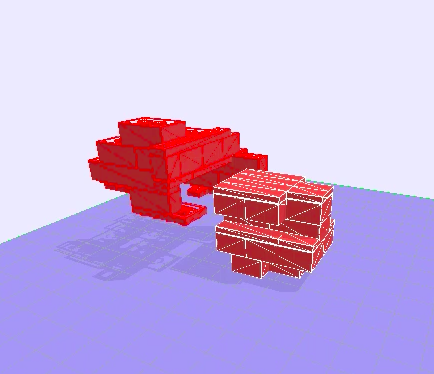
\includegraphics[width=.5\textwidth]{./figures/bullet_demo.png}
  \caption{Tool and object models loaded into Bullet simulation demo}
  \label{fig:bullet_demo}
\end{figure}      

We test Bullet's collision detection in a demo containing simple tool and object models (fig. \ref{fig:bullet_demo}).
The passive object is first set on a flat surface.
Following, the tool is positioned to slid into the object's fitting and lift it.
Demo code is therefore representative of the real-world experiment.  

A magnitude of parameters can influence the effects of interaction between the two objects:
\begin{enumerate}
  \item Object collision properties are most commonly represented by classes which approximate the object's shape in order to gain execution speed.
    A more precise approach is to use classes that represent the object's true collision shape (fig. \ref{fig:collision_shape}).   

\begin{figure}[h]
  \centering
  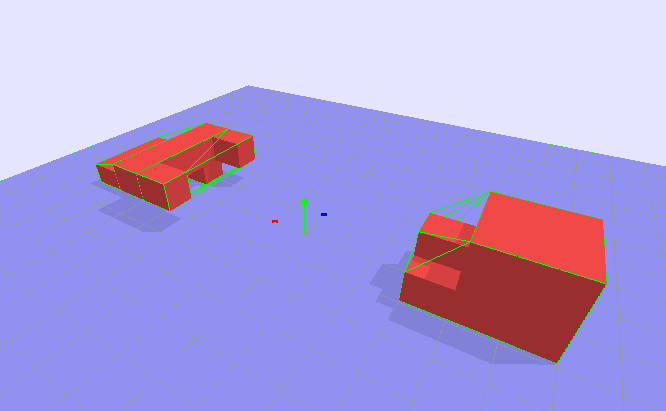
\includegraphics[width=.48\textwidth]{./figures/collision_approximation.png}
  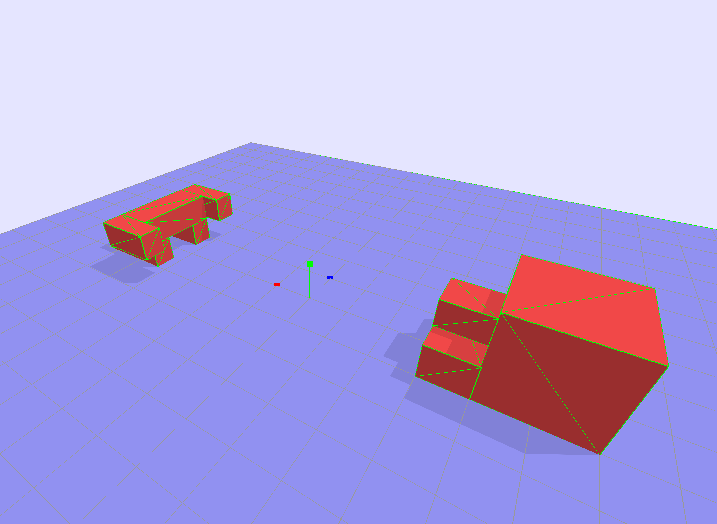
\includegraphics[width=.41\textwidth]{./figures/collision_exact.png}
  \caption{Comparison of approximated collision and exact collision shape}
  \label{fig:collision_shape}
\end{figure}      

  \item A threshold or margin of contact exists between objects. When the margin is to low, shaking effects can be noticed as the objects make contact. Alternatively, when the margin is too large, the object's collision would not be representative of geometry. 

  \item Moving the tool to interact with the object can be done in multiple ways, each with different degrees of realism.
\end{enumerate}

From a development perspective, the engine was easy to build and has detailed documentation.
Matlab integration is also available from 3rd party developers. 
However, the integration layer is not well maintained having missing functionality or failing to build.
A model using Bullet Physics would therefore have to be developed in C++. 

Overall Bullet Physics suffers from a high degree of shaking when tool and object interact. 
As the object is within the grasp of the tool, collision points make the object bounce uncontrollably within the tool's clamp. As bounce forces amplify the target object eventually bursts out of the tool's fixation.  
Parameters of the engine can be tuned to minimise the effects, but would ultimately lead to less representative tool use simulations. 

\subsection{Newton Game Dynamics}
Newton Game Dynamics is regarded as having better precision than Bullet, but at the cost of performance \cite{hummel2012}. 
The precision gain is achieved by using a deterministic solver instead of numerical methods for integrating movement and forces over time. 

\begin{figure}[h]
  \centering
  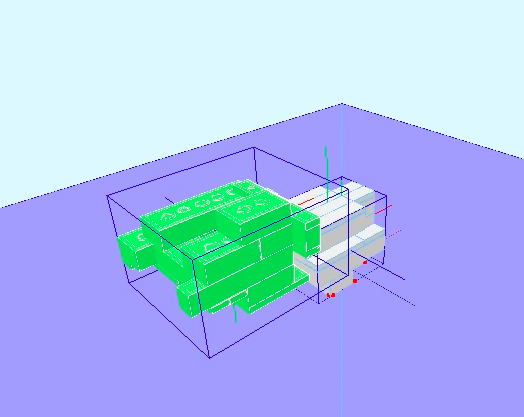
\includegraphics[width=.5\textwidth]{./figures/newton_demo.png}
  \caption{Tool and object models loaded into Bullet simulation demo}
  \label{fig:newton_demo}
\end{figure}      

We setup a demo similar to the Bullet one.
The object is set on a flat surface. 
The tool is then slid into object's fitting and lifted (\ref{fig:newton_demo}). 

Compared to Bullet, Newton's default behaviour shows realistic behaviour. 
The simulation exhibits no shaking or other unrealistic effects.
The tool and object move smoothly on established trajectories. 

From a development point of view, Newton lacks the quality of documentation found in Bullet. 
There are thousands of lines of example code available, but locating needed functionality is difficult. 
This is made worse by a strange, yet consistent API interaction.

Additionally, the engine supports unconventional 3D file formats, making it difficult to load item models.
Code has to be developed to support more common file formats.

As a less popular engine, Newton does not have integration with other languages (e.g. Matlab or Python). 
A computational model would have to be written in C++.

Even with the above development concerns, the engine's simulation precision make it the prime candidate for our model.  

\section{Exhaustive Search}
Demos show how tool-object fitting can be verified through simulation.
As the model aims to solve fitting problems, one can position items in all possible configurations to select valid ones. 
Validity implies that the tool can lift the object, and that models do not penetrate each other's surface.
A configuration represents a tool's rotation and relative position to the object.
That is X,Y,Z coordinates and rotations around each axis (i.e. yaw, pitch, roll). 
An \emph{Exhaustive Search} model outputs solutions by testing all possible configurations.

\subsection{Implementation Details}
The target object is positioned on a flat surface. 
The tool is then placed in successive relative locations, and object collision is tested. 
For any collision points to be detected, one simulation time step has to be executed.
Newton Physics allows obtaining the penetration depth of collision points. 
When penetration is too high, the configuration is deemed invalid. 

If penetration depth is zero, the object and tool may not be in contact at all. 
To invalidate such scenarios, a lifting force is applied to the tool.
When the objects are in contact, lifting velocity would transfer to the target object and may be asserted. 

The approach is able to verify a single fitting configuration per physics engine update step.
However, as object contact is detected through a small penetration margin it is possible that undesired vertical forces appear.
As a result output data would contain invalid solutions which require further validation.

Physics engines do not require 3D rendering when computing object dynamics. 
The exhaustive search can run in either graphical or non-graphical mode.
Graphical rendering allows researchers to investigate the correct loading of objects and interactions in the 3D world.
The non-graphical model allows faster computation as rendering overburden is removed. 

\begin{figure}[h]
  \centering
  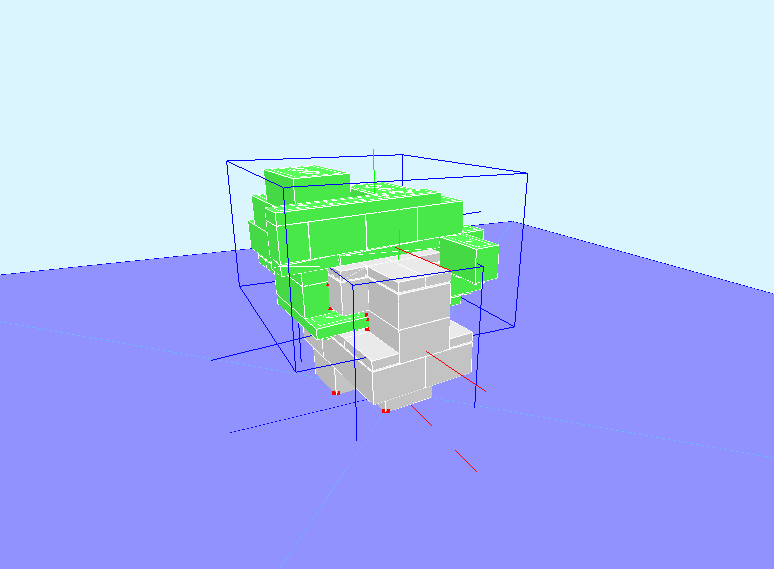
\includegraphics[width=.7\textwidth]{./figures/newton_simulation.png}
  \caption{Exhaustive search rendering}
  \label{fig:newton_simulation}
\end{figure}      

Figure \ref{fig:newton_simulation} captures the rendering of two objects in fitting position.
Visual meshes are displayed in green.
Collision meshes are outlined by white lines.
Contact points are displayed as red dots.
3D orientation vectors give visual queues of rotation angles (red, green, blue for X, Y, Z respectively).
Blue bounding boxes represent vertex extremities (i.e. min and max X, Y, Z coordinates).
 
Newton dynamics has the in built ability to optimise meshes as convex decomposition.
This means, complex assemblies of triangles representing simple shapes can be optimised to simpler mesh structures representing the same shapes. 
A complex object would therefore be transformed to an assembly of simple shapes, optimising collision detection and computation. 

\subsection{Discussion}
When search intervals are in the vicinity of possible solutions, the model finds multiple equivalent fitting configurations.
However, on a single multi-core computer the exhaustively searching is unfeasible. 
The tool's position is determined by 6 dimensions of freedom amounting to $~10^12$ possible configurations. 
Even for a single tool rotation there are $~10^8$ configurations which require an hour of execution to verify. 

As described in the implementation, verifying configurations has been optimised for speed.
Further improvements can be achieved by splitting the search space over multiple machines.
Alternatively, the search step can be increased at the expense of missing possible solutions. 

%unrealistic representation of human behaviour
Exhaustively searching is lengthy and computationally expensive.
Engine features, such as penetration depth, can be leveraged by more ingenious search algorithms.
However, solutions based solely on the engine's functionality remain problematically unrealistic of physical laws and human ability.
For example, the tool can be positioned to lift an object even when no physical manner would allow it to be placed in that location.  

There is also a question of how a subject may grasp the tool.
During simulations, lifting forces are applied to the tool's center of gravity.
The search may therefore produce fittings that do not realistically permit the tool to be held.

%motivation for a heuristic search
Computational expense yet remains the impeding factor to the model's use. 
Heuristic methods can be used to optimise the search problem, whilst better resembling human ability.
However, physics simulations remain a viable approach to verifying solutions. 

\printbibliography
\end{document}
